\documentclass[10pt,spanish,aspectratio=1610]{beamer}
\usepackage[utf8]{inputenc}
\usepackage{amsmath}
\usepackage{graphicx}
\usepackage{amssymb}
\usepackage[spanish]{babel}
\spanishdecimal{.}
\usepackage{subfig}
\usepackage{fancyhdr}
\usepackage{pstricks}
\usepackage{color}
\usepackage[ruled]{algorithm2e}
\usepackage{listings}
\usepackage{multicol}
\usepackage{xcolor}

\definecolor{graywhite}{rgb}{0.9529,0.9607,0.9686}
\definecolor{bluegray}{rgb}{0.6823, 0.7411, 0.8}
\definecolor{darkred}{rgb}{0.7372, 0.2392, 0.2392}
\definecolor{bluedark}{rgb}{0.294, 0.4705, 0.6407}
\definecolor{darkgreen}{rgb}{0.1764, 0.5294, 0.0901}
\lstset{
  backgroundcolor=\color{graywhite},   % choose the background color; you must add \usepackage{color} or \usepackage{xcolor}; should come as last argument
  basicstyle=\footnotesize,        % the size of the fonts that are used for the code
  breakatwhitespace=false,         % sets if automatic breaks should only happen at whitespace
  breaklines=true,                 % sets automatic line breaking
  captionpos=b,                    % sets the caption-position to bottom
  commentstyle=\color{darkgreen},    % comment style
  keepspaces=true,                 % keeps spaces in text, useful for keeping indentation of code (possibly needs columns=flexible)
  keywordstyle=\color{darkred},       % keyword style
  language=Octave,                 % the language of the code
  morekeywords={*,...},            % if you want to add more keywords to the set
  numbers=left,                    % where to put the line-numbers; possible values are (none, left, right)
  numbersep=7pt,                   % how far the line-numbers are from the code
  numberstyle=\tiny\color{bluedark}, % the style that is used for the line-numbers
  showspaces=false,                % show spaces everywhere adding particular underscores; it overrides 'showstringspaces'
  showstringspaces=false,          % underline spaces within strings only
  showtabs=false,                  % show tabs within strings adding particular underscores
  stepnumber=1,                    % the step between two line-numbers. If it's 1, each line will be numbered
  stringstyle=\color{bluedark},     % string literal style
  frame=single,
  rulecolor=\color{bluegray},
  tabsize=2,                   % sets default tabsize to 2 spaces
  xleftmargin=1cm,
  xrightmargin=0.5cm,
  framexleftmargin=0.5cm,
  extendedchars=true,
  literate={á}{{\'a}}1 {é}{{\'e}}1 {í}{{\'i}}1 {ó}{{\'o}}1 {ú}{{\'u}}1 {Á}{{\'A}}1 {É}{{\'E}}1 {Í}{{\'I}}1 {Ó}{{\'O}}1 {Ú}{{\'U}}1,
}

\DeclareMathOperator{\atantwo}{atan2}
\setbeamercolor{block title}{fg=white,bg=blue!70!black}
\setbeamercolor{block body}{fg=black, bg=blue!10!white}
\setbeamertemplate{blocks}[rounded][shadow=false]
\setbeamercovered{transparent}
\beamertemplatenavigationsymbolsempty
\setbeamertemplate{frametitle}{
  \leavevmode
  \hbox{\begin{beamercolorbox}[wd=0.85\paperwidth,left]{frametitle}
    \usebeamerfont{frametitle}\insertframetitle
  \end{beamercolorbox}
%  \begin{beamercolorbox}[wd=0.25\paperwidth,center]{frametitle}
%    \usebeamerfont{frametitle}\hfill\hspace*{5ex}\footnotesize{\insertsubsection}
%  \end{beamercolorbox}
}}
\setbeamertemplate{footline}{
  \leavevmode%
  \hbox{%
    \begin{beamercolorbox}[colsep=-0.5pt,wd=.33\paperwidth,ht=3ex,dp=1.5ex,center]{author in head/foot}%
      \usebeamerfont{author in head/foot}\insertshortauthor~~ (\insertshortinstitute)
    \end{beamercolorbox}%
    \begin{beamercolorbox}[colsep=-0.5pt,wd=.34\paperwidth,ht=3ex,dp=1.5ex,center]{date in head/foot}%
      \usebeamerfont{author in head/foot}\insertshorttitle
    \end{beamercolorbox}%
    \begin{beamercolorbox}[colsep=-0.5pt,wd=.33\paperwidth,ht=3ex,dp=1.5ex,right]{author in head/foot}%
      \usebeamerfont{author in head/foot}\insertshortdate{} \hspace*{2em}\scriptsize{\insertframenumber{}}\hspace*{1ex}
    \end{beamercolorbox}
  }
}
\setbeamersize
{
    text margin left=0.25cm,
    text margin right=0.25cm
}

\begin{document}
\renewcommand{\tablename}{Tabla}
\renewcommand{\figurename}{Figura}

\title[Vehículos autónomos y la liga AutoModelCar]{Comportamientos para vehículos autónomos y la categoría AutoModelCar}
\author[Marco Negrete]{Instructor: Dr. Marco Antonio Negrete Villanueva}
\institute[FI, UNAM]{Facultad de Ingeniería, UNAM}
\date[EIR 2024]{Escuela de Invierno de Robótica 2024\\Nanchital, Veracruz\\\url{https://github.com/mnegretev/EIR-2024-AutonomousVehicles}}

\begin{frame}
\titlepage
\end{frame}

\begin{frame}
  \Large{Objetivos:}
  \normalsize
  \[\]
  \textbf{Objetivo General:} Revisar conceptos básicos para operar un vehículo sin conductor en el contexto de las pruebas de la categoría AutoModelCar
  \\
  \textbf{Objetivos Específicos:}
  \begin{itemize}
  \item Revisar el hardware necesario para tener un vehículo sin conductor
  \item Dar un panorama general del software necesario para desarrollar un vehículo sin conductor
  \item Revisar las herramientas disponibles para implementar los comportamientos básicos en un vehículo sin conductor
    \begin{itemize}
    \item Detección de carriles
    \item Seguimiento de carriles
    \item Rebase
    \item Detección de señales de tránsito
    \end{itemize}
  \end{itemize}
\end{frame}

\begin{frame}
  \Large{Contenido}
  \normalsize
  \[\]

  \tableofcontents
\end{frame}

\section{Introducción}

\begin{frame}\frametitle{Motivación}
  ¿Por qué vehículos sin conductor?
  \begin{itemize}
  \item La mayor cantidad de accidentes tienen como causa un error humano
  \item Se podría disminuir este número con vehículos sin conductor
  \item Menores tiempos de traslado mediante planeación de rutas óptimas y conducción sin distracciones
  \item Movilidad urbana más accesible
  \item Disminución de emisiones debido a una conducción óptima
  \end{itemize}
\end{frame}

\begin{frame}\frametitle{¿Cuándo un vehículo se considera autónomo?}
  La SAE propone seis niveles de autonomía:
  \[\]
  \textbf{Nivel 0 (\textit{No driving automation}):} El conductor es responsable de todas las tareas de conducción.
  \[\]
  \textbf{Nivel 1 (\textit{Driving assistance}):} El sistema de conducción automatizada toma control en situaciones muy específicas. Ejemplo: mantener cierta velocidad en carretera o frenar en automático ante un obstáculo.
  \begin{figure}
    \centering
    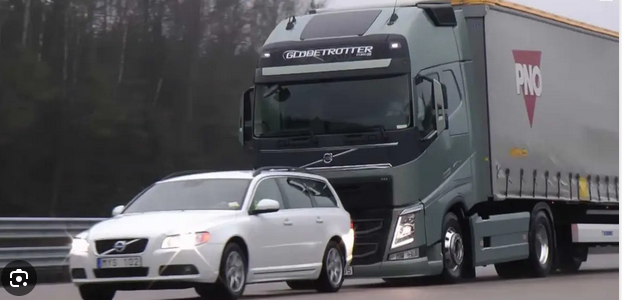
\includegraphics[width=0.5\textwidth]{Figuras/EjemploSAE1.png}
  \end{figure}
\end{frame}

\begin{frame}\frametitle{Niveles de autonomía SAE}
  \textbf{Nivel 2 (\textit{Partial driving automation}):} El auto puede realizar la mayor parte de tareas de conducción pero el conductor debe mantenerse atento durante toda la conducción. Ejemplo: Tesla.
  \begin{figure}
    \centering
    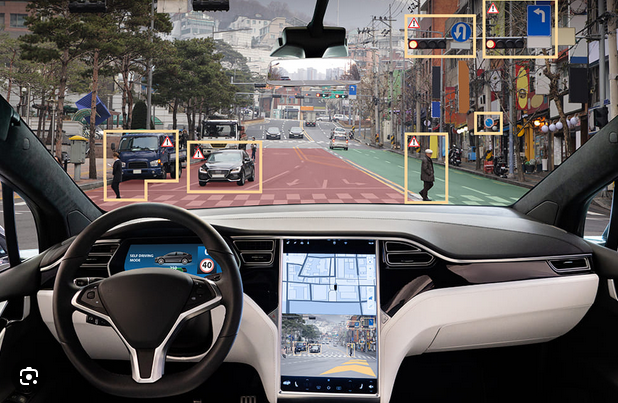
\includegraphics[width=0.5\textwidth]{Figuras/EjemploSAE2.png}
  \end{figure}
\end{frame}

\begin{frame}\frametitle{Niveles de autonomía SAE}
  \textbf{Nivel 3 (\textit{Conditional driving automation}):} El conductor puede desconectarse de la tarea de conducción bajo ciertos climas y carreteras. Todavía se requiere que el conductor resuelva ciertas situaciones de manejo. Ejemplo: Mercedes-Benz
  \begin{figure}
    \centering
    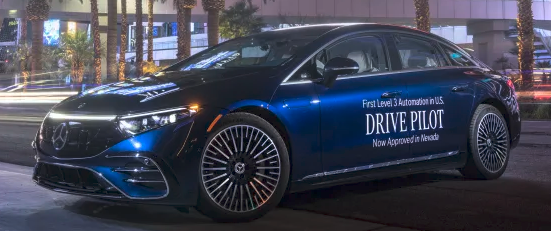
\includegraphics[width=0.7\textwidth]{Figuras/EjemploSAE3.png}
  \end{figure}
\end{frame}

\begin{frame}\frametitle{Niveles de autonomía SAE}
  \textbf{Nivel 4 (\textit{High driving automation}):} El vehículo es capaz de ejecutar funciones tácticas y operativas y es capaz de asegurarse automáticamente si los límites operativos se superan. El vehículo no es completamente autónomo pero el conductor no necesita responder ante fallas operativas. Ejemplo: \textbf{El TMR, pronto (esperemos)}
  \[\]
  \textbf{Nivel 5 (\textit{Full driving automation}):} No se requiere intervención humana y el sistema puede conducir sin restricciones de clima, carretera, horario o condición geográfica.  Ejemplo: \textbf{El TMR, pronto (esperemos)}
\end{frame}

\begin{frame}\frametitle{Software requerido}
  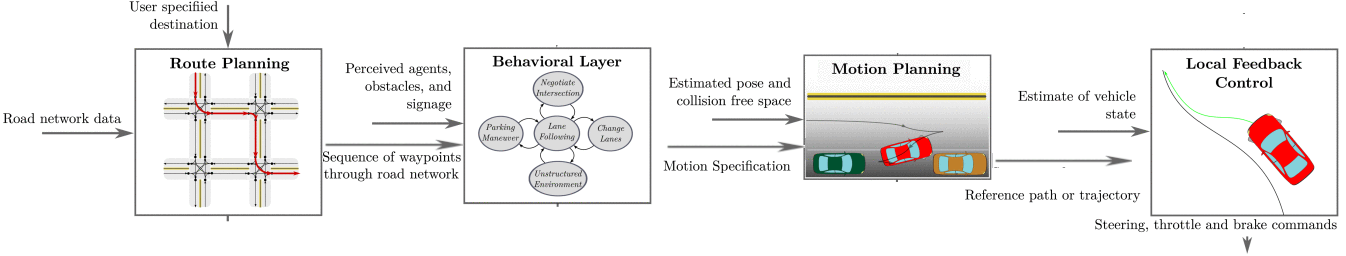
\includegraphics[width=\textwidth]{Figuras/SoftwareArchitecture.png}
  (Imagen tomada de \textit{A Survey of Motion Planning and Control Techniques for Self-Driving Urban Vehicles})
\end{frame}

\begin{frame}\frametitle{Propuesta para selección de comportamientos}
  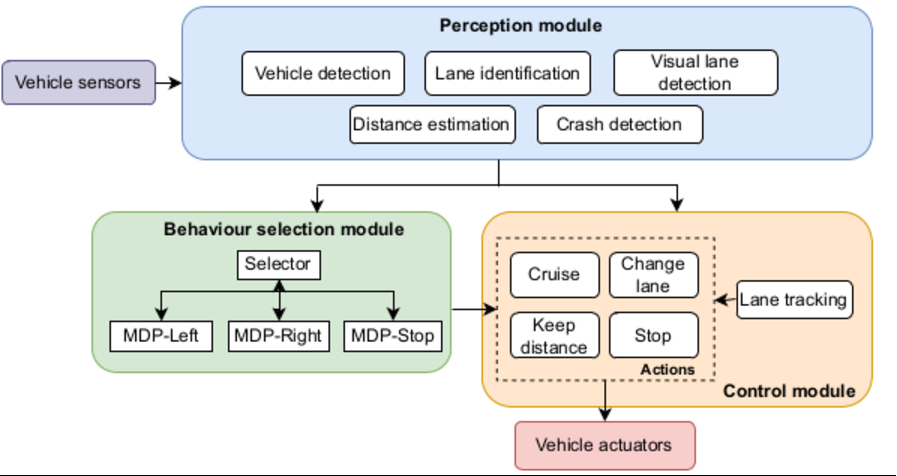
\includegraphics[width=\textwidth]{Figuras/GeneralArchitecture.pdf}
\end{frame}
\section{La plataforma ROS}
\begin{frame}\frametitle{La plataforma ROS}
  
\includegraphics[width=0.3\textwidth]{Figuras/Ros_logo.png}
  \[\]
  \textbf{ROS (Robot Operating System) } es un \textit{middleware} de código abierto para el desarrollo de robots móviles.
  \begin{itemize}
  \item Implementa funcionalidades comúnmente usadas en el desarrollo de robots como el paso de mensajes entre procesos y la administración de paquetes.
  \item Muchos drivers y algoritmos ya están implementados.
  \item Es una plataforma distribuida de procesos (llamados \textit{nodos}).
  \item Facilita el reuso de código.
  \item Independiente del lenguaje (Python y C++ son los más usados).
  \item Facilita el escalamiento para proyectos de gran escala. 
  \end{itemize}
\end{frame}

\begin{frame}\frametitle{Conceptos}
  ROS se puede entender en dos grandes niveles conceptuales:
  \begin{itemize}
  \item \textbf{Sistema de archivos:} Recursos de ROS en disco
  \item \textbf{Grafo de procesos:} Una red \textit{peer-to-peer} de procesos (llamados nodos) en tiempo de ejecución.
  \end{itemize}
\end{frame}

\begin{frame}\frametitle{Sistema de archivos}
  \begin{columns}
    \begin{column}{0.5\textwidth}
      Recursos en disco:
      \begin{itemize}
      \item \textbf{Workspace:} carpeta que contiene los paquete desarrollados
      \item \textbf{Paquetes:} Principal unidad de organización del software en ROS (concepto heredado de Linux)
      \item \textbf{Manifiesto:} (\texttt{package.xml}) provee metadatos sobre el paquete (dependencias, banderas de compilación, información del desarrollador)
      \item \textbf{Mensajes (msg):} Archivos que definen la estructura de un \textit{mensaje} en ROS.
        \item \textbf{Servicios (srv):} Archivos que definen las estructuras de la petición (\textit{request}) y respuesta (\textit{response}) de un servicio. 
      \end{itemize}
    \end{column}
    \begin{column}{0.4\textwidth}
      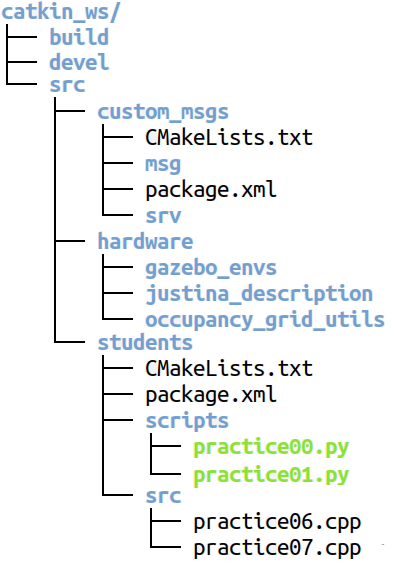
\includegraphics[width=\textwidth]{Figuras/catkin_tree.png}
    \end{column}
  \end{columns}
\end{frame}

\begin{frame}\frametitle{Grafo de procesos}
  El grafo de procesos es una red \textit{peer-to-peer} de programas (nodos) que intercambian información entre sí. Los principales componentes del este grafo son:
  \[\]
  \begin{columns}
    \begin{column}{0.5\textwidth}
      \begin{itemize}
      \item master
      \item servidor de parámetros
      \item nodos
      \item mensajes
      \item servicios 
      \end{itemize}
    \end{column}
    \begin{column}{0.5\textwidth}
      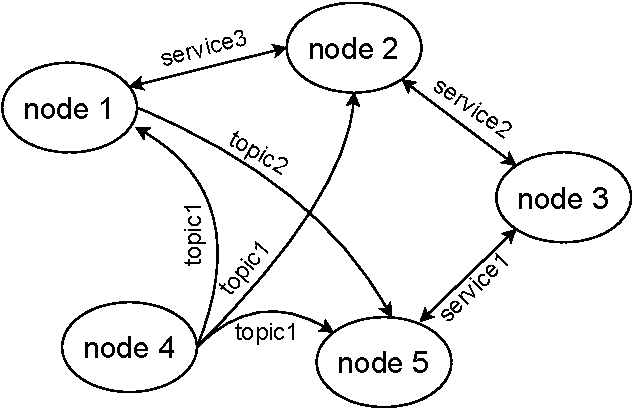
\includegraphics[width=\textwidth]{Figuras/RosGraph.pdf}
    \end{column}
  \end{columns}
\end{frame}

\begin{frame}\frametitle{Tópicos y servicios}
  Los nodos (procesos) en ROS intercambian información a través de dos grandes patrones:
  \begin{columns}
    \begin{column}{0.6\textwidth}
        \begin{itemize}
        \item \textbf{Tópicos}
          \begin{itemize}
          \item Son un patrón $1:n$ de tipo \textit{publicador/suscriptor}
          \item Son no bloqueantes
          \item Utilizan estructuras de datos definidas en archivos \texttt{*.msg} para el envío de información
          \end{itemize}
        \item \textbf{Servicios}
          \begin{itemize}
          \item Son un patrón $1:1$ de tipo \textit{petición/respuesta}
          \item Son bloqueantes
          \item Utilizan estructuras de datos definidas en archivos \texttt{*.srv} para el intercambio de información. 
          \end{itemize}
        \end{itemize}
    \end{column}
    \begin{column}{0.4\textwidth}
      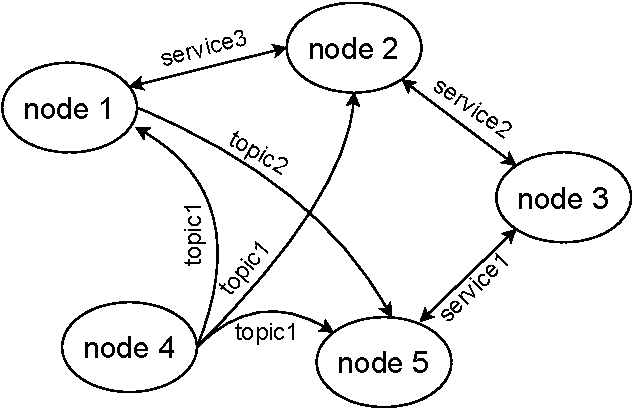
\includegraphics[width=\textwidth]{Figuras/RosGraph.pdf}
    \end{column}
  \end{columns}
  \[\]
  Para mayor información:
  \begin{itemize}
  \item Tutoriales \url{http://wiki.ros.org/ROS/Tutorials}
  \item Koubâa, A. (Ed.). (2020). Robot Operating System (ROS): The Complete Reference. Springer Nature
  \end{itemize}
\end{frame}

\section{La categoría AutoModelCar}

\begin{frame}\frametitle{La categoría AutoModelCar}
  \begin{itemize}
  \item Se originó por el proyecto \textit{Visiones de movilidad urbana} a través del cual se donaron vehículos a escala a varias instituciones educativas y de investigación del país
    \begin{figure}
      \centering
      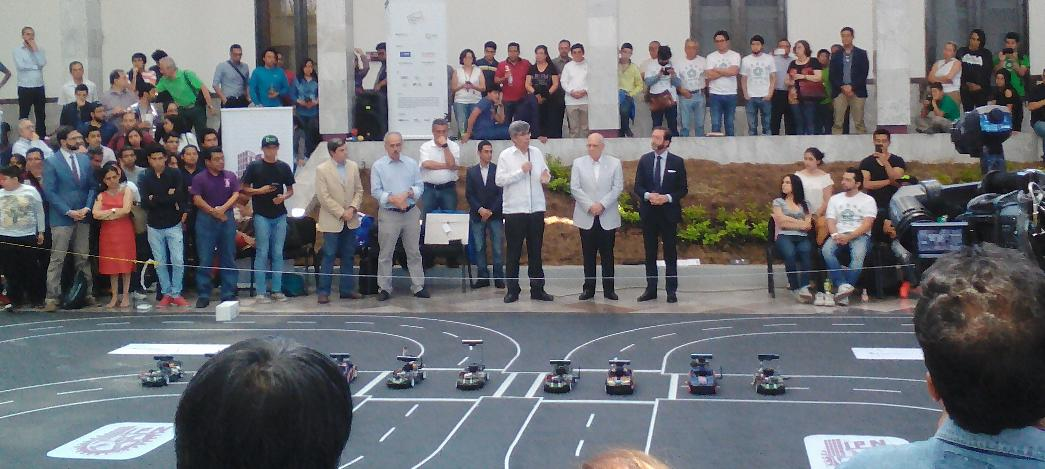
\includegraphics[width=0.9\textwidth]{Figuras/VisionesDeMovilidadUrbana.jpg}
    \end{figure}
  \end{itemize}
\end{frame}

\begin{frame}\frametitle{La categoría AutoModelCar}
  \begin{itemize}
  \item Originalmente solo se permitían vehículos AutoNOMOS:
    \begin{figure}
      \centering
      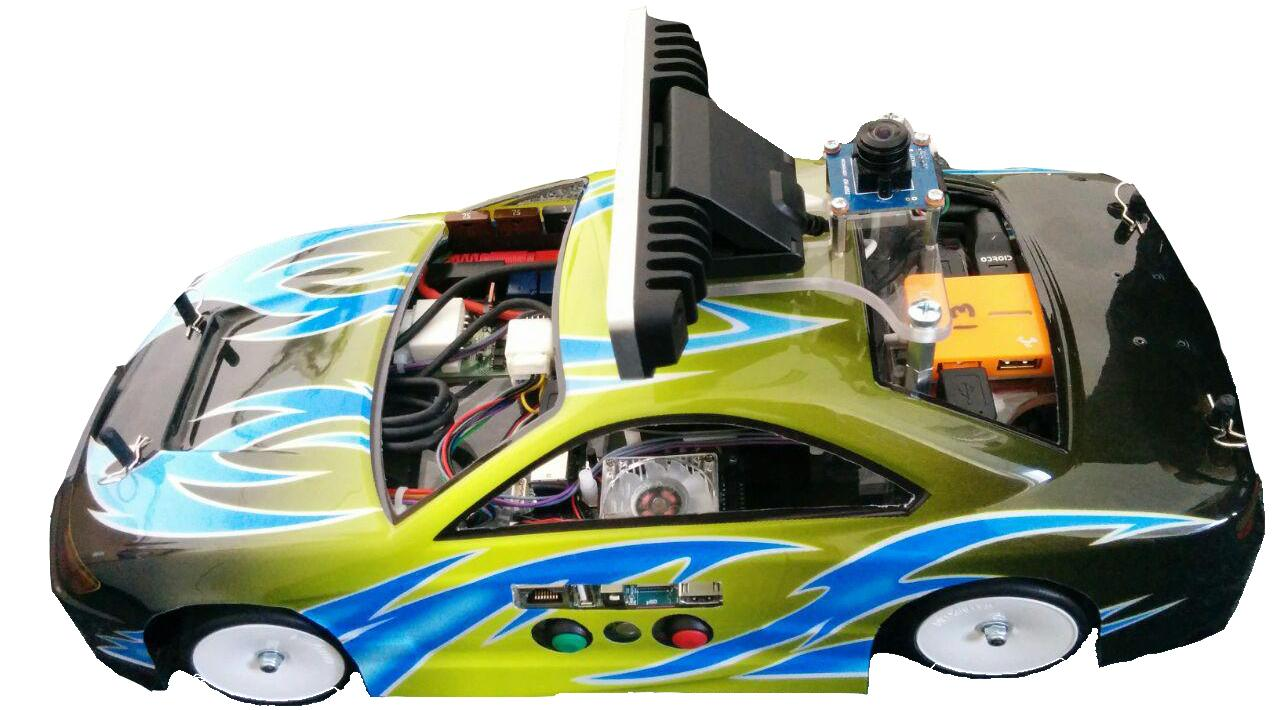
\includegraphics[width=0.35\textwidth]{Figuras/AutoNOMOS.jpg}
    \end{figure}
  \item Pero ahora se puede participar con cualquier vehículo a escala:
    \begin{figure}
      \centering
      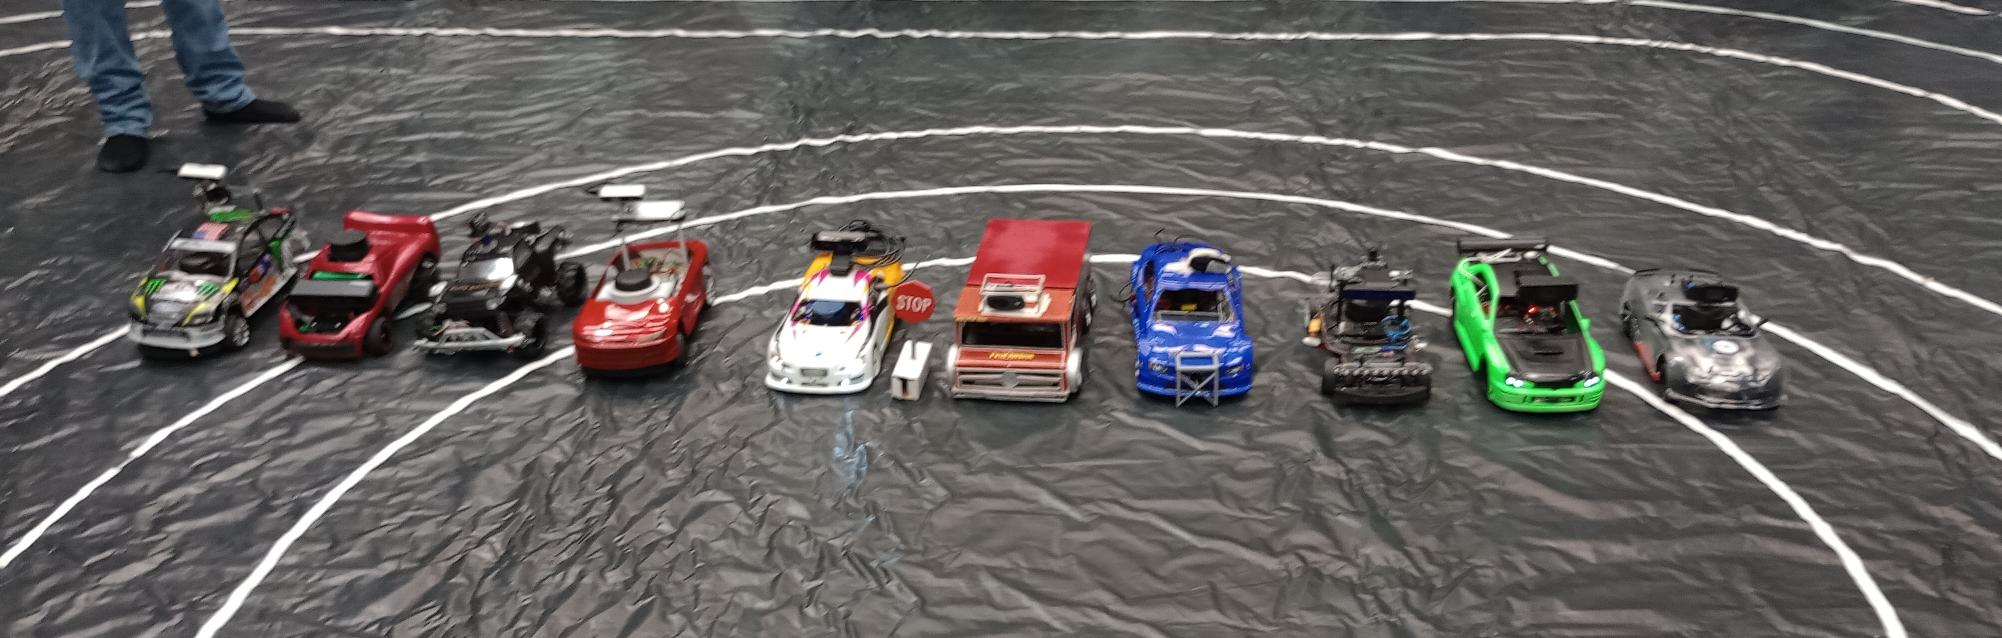
\includegraphics[width=0.75\textwidth]{Figuras/AutoModelCarCars.jpg}
    \end{figure}
  \end{itemize}
\end{frame}

\begin{frame}\frametitle{La categoría AutoModelCar}
  \begin{itemize}
  \item La competencia consta de cuatro pruebas (esperemos aumentarlas este año):
    \begin{multicols}{2}
      \begin{itemize}
      \item Navegación autónoma sin obstáculos
      \item Navegación con obstáculos estáticos
      \item Navegación con obstáculos en movimiento
      \item Estacionamiento
      \end{itemize}
    \end{multicols}
    \begin{figure}
      \centering
      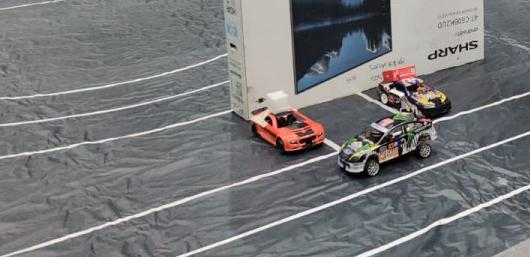
\includegraphics[width=0.6\textwidth]{Figuras/AutoModelCarEstacionamiento.jpg}
    \end{figure}
  \end{itemize}
\end{frame}

\begin{frame}\frametitle{La categoría AutoModelCar}
  Se utiliza una pista con rectas, curvas y cruces:
  \begin{figure}
    \centering
    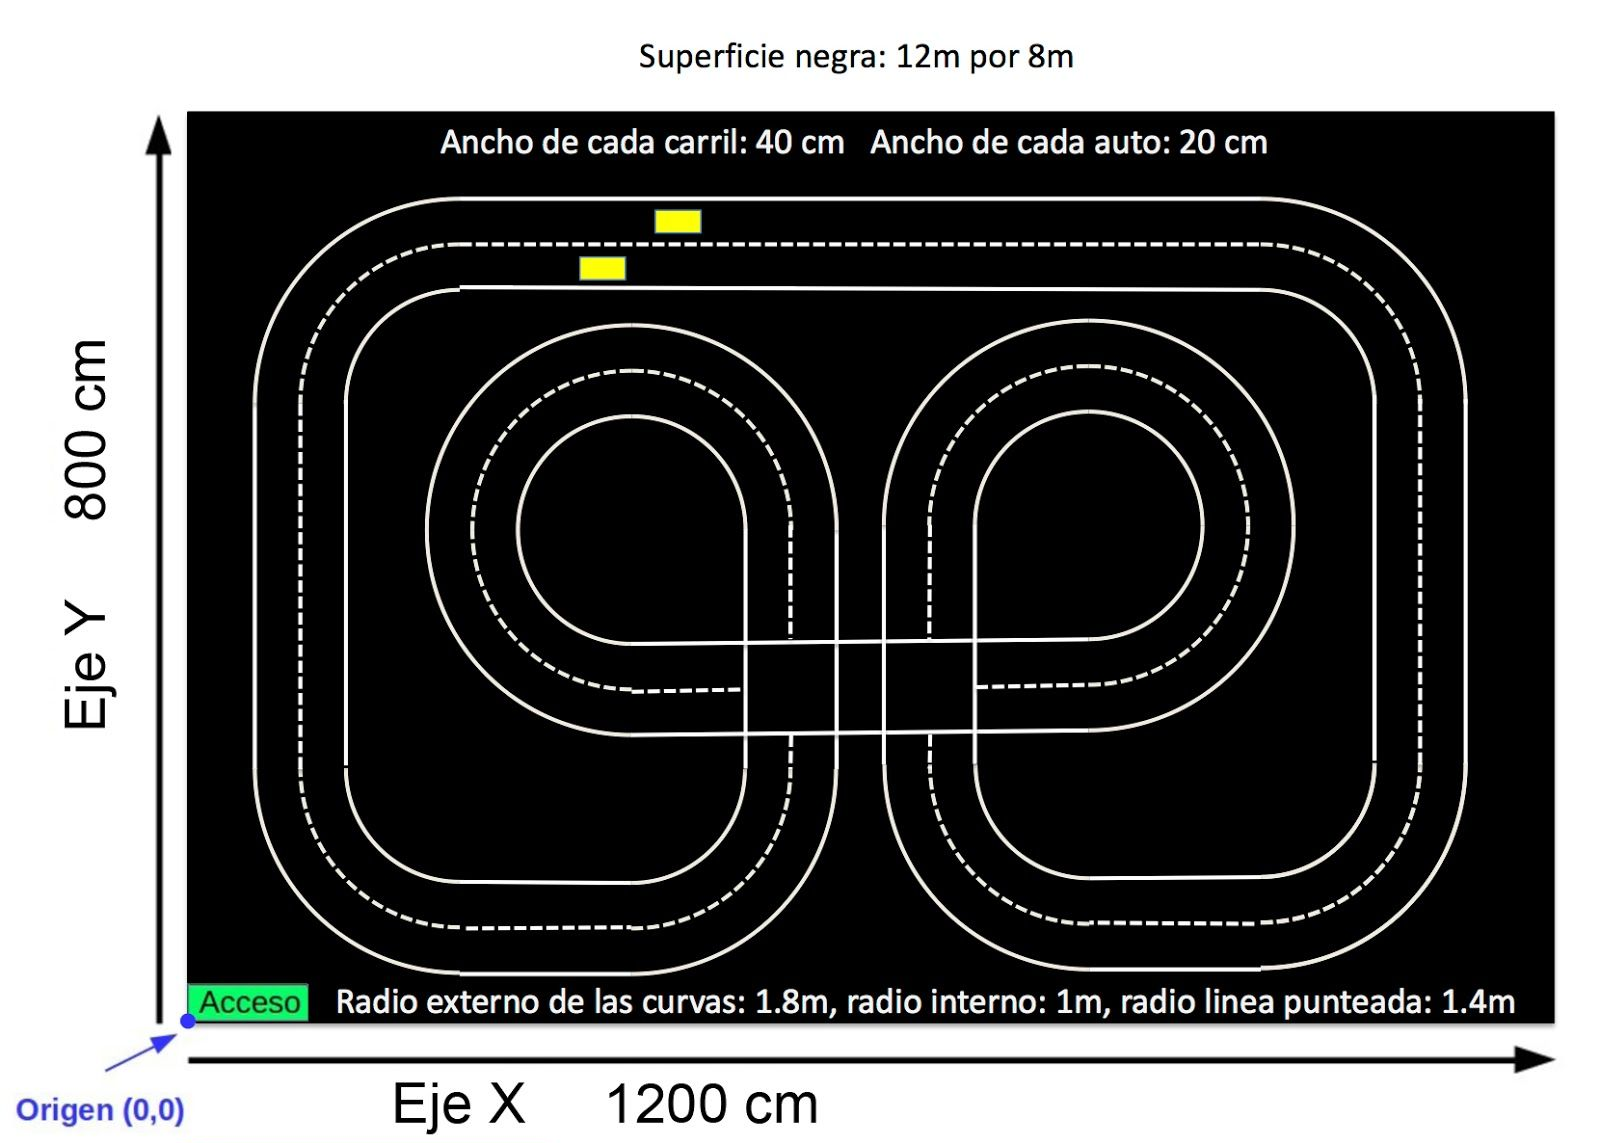
\includegraphics[width=0.7\textwidth]{Figuras/AutoModelCarPista.png}
  \end{figure}
\end{frame}

\begin{frame}\frametitle{Hardware para vehículos sin conductor}
  \begin{figure}
    \centering
    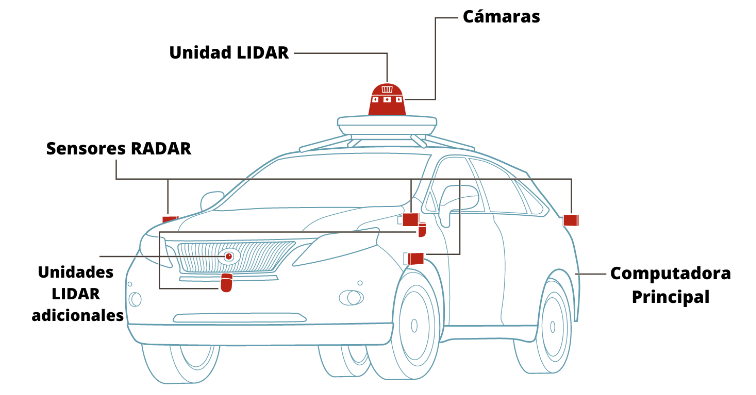
\includegraphics[width=0.6\textwidth]{Figuras/Hardware.png}
  \end{figure}
\end{frame}

\begin{frame}\frametitle{Herramientas de simulación}
  ¿Por qué utilizar simuladores?
  \begin{itemize}
  \item Instrumentar un vehículo autónomo puede ser costoso, incluso si se hace a escala.
  \item En simulación se pueden construir ambientes controlados que permiten probar partes específicas del sistema de autonomía.
  \item Se pueden enfocar los esfuerzos al desarrollo de software dando por hecho un hardware funcional.
  \item Algunos ejemplos de simuladores:
    \begin{itemize}
    \item Gazebo (utilizado en el TMR 2021)
    \item Webots (utilizado en los TMRs 2022 y 2023)
    \item Matlab (utilizado por quien tiene dinero para pagar la licencia)
    \end{itemize}
  \end{itemize}
\end{frame}

\begin{frame}\frametitle{El simulador Webots}
  El simulador Webots tiene varias características para simulación de vehículos sin conductor:
  \begin{itemize}
  \item Motor de físicas ODE y OpenGL como motor de renderizado.
  \item Multiplataforma y disponible para sistemas operativos Linux, Windows y macOS.
  \item Programación en diferentes lenguajes: C, C++, Python, Java, MATLAB.
  \item Amplía variedad de robots, sensores, actuadores, objetos y materiales.
  \item Fácil integración con la plataforma ROS.
  \end{itemize}
  \begin{figure}
    \centering
    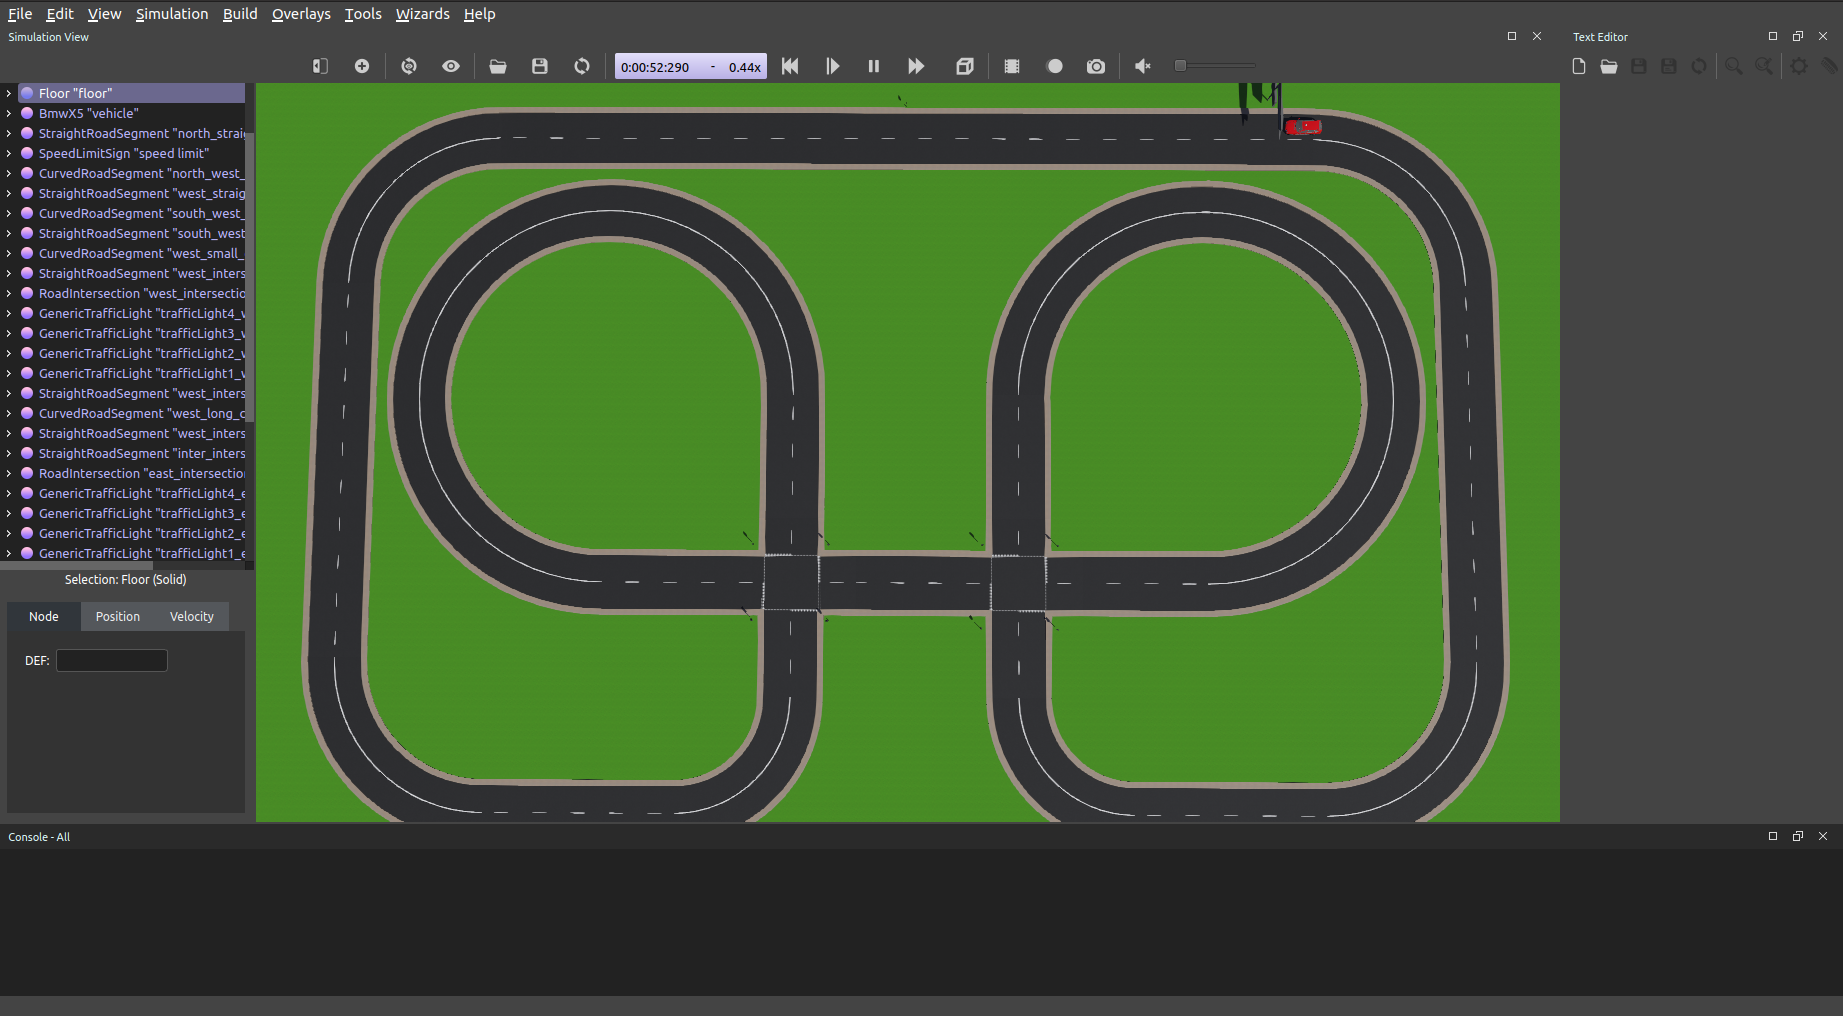
\includegraphics[width=0.7\textwidth]{Figuras/WebotsExample.png}
  \end{figure}
\end{frame}

\begin{frame}\frametitle{SUMO (Simulation of Urban Mobility)}
  Es un paquete de simulación de tráfico desarrollado por el Centro Aeroespacial Alemán.
  \begin{itemize}
  \item De código abierto
  \item Diseñado para manejar redes grandes de vehículos
  \item Se pueden simular vehículos, peatones, ciclistas, señales de tránsito, transporte público, entre muchas otras opciones
  \item Fácil intregración con Webots mediante el objeto \textit{SUMO interface}:
  \item Se puede definir el comportamiento de los vehículos mediante archivos \texttt{*.nod.xml}, \texttt{*.edg.xml}, \texttt{*.net.xml}, \texttt{*.rou.xml} y \texttt{*.sumocfg}
  \end{itemize}
\end{frame}

\begin{frame}[containsverbatim]\frametitle{Ejercicio 1 - Herramientas de simulación}
  \begin{enumerate}
  \item Abra una terminal y ejecute la simulación con el comando:
    \begin{lstlisting}[language=bash,numbers=none]
roslaunch eir2024 navigation_moving_obstacles.launch
    \end{lstlisting}
  \item Detenga la simulación
  \item Abra el archivo \texttt{catkin\_ws/src/eir2024/worlds/navigation\_moving\_obstacles\_net/sumo.rou.xml} y descomente las líneas 8 a 14
  \item Corra nuevamente la simulación. Se deberían observar más vehículos
  \item Detenga la simulación y ejecute los siguientes comandos:
    \begin{lstlisting}[language=bash,numbers=none]
roscd eir2024/worlds/navigation_moving_obstacles_net/
netconvert -S 10 -n sumo.nod.xml -e sumo.edg.xml -o sumo.net.xml
    \end{lstlisting}
  \item Corra nuevamente la simulación. Se debería notar un cambio en la velocidad de los vehículos
  \end{enumerate}
\end{frame}

\section{Detección de carriles}

\begin{frame}\frametitle{Imágenes como funciones}
  \begin{itemize}
  \item Una imagen (en escala de grises) es una función $I(x,y)$ donde $x,y$ son variables discretas en coordenadas de imagen y la función $I$ es intensidad luminosa.
    \item Las imágenes también pueden considerarse como arreglos bidimensionales de números entre un mínimo y un máximo (usualmente 0-255).
    \item Aunque formalmente una imagen es un mapeo $f:\mathbb{R}^2\rightarrow \mathbb{R}$, en la práctica, tanto $x,y$ como $I$ son varialbes discretas con valores entre un mínimo y un máximo.
    \item Las imágenes de color son funciones vectoriales $f:\mathbb{R}^2\rightarrow \mathbb{R}^3$ donde cada componente de la función se llama canal.
%  \[I(x,y) = \left[\begin{tabular}{c}$r(x,y)$\\$g(x,y)$\\$b(x,y)$\end{tabular}\right]\]
  \end{itemize}
  \begin{figure}
    \centering
    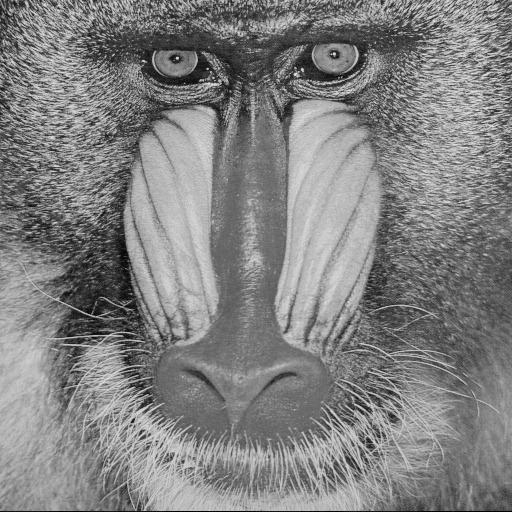
\includegraphics[width=0.3\textwidth]{Figuras/BaboonGrayscale.jpg}
    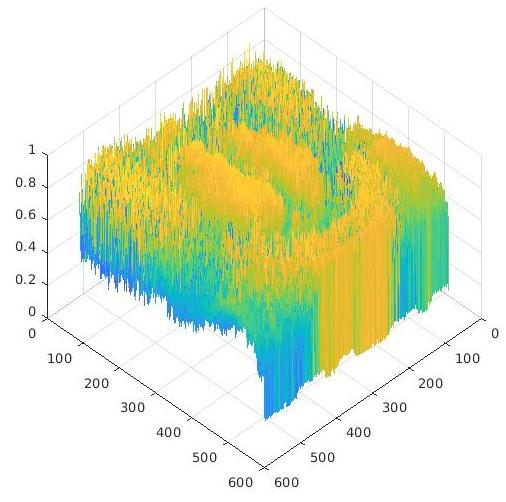
\includegraphics[width=0.35\textwidth]{Figuras/BaboonPlot.jpg}
  \end{figure}
\end{frame}

\begin{frame}\frametitle{OpenCV}
  \begin{columns}
    \begin{column}{0.5\textwidth}
      \begin{figure}
        \centering
        
\includegraphics[width=0.6\textwidth]{Figuras/OpenCVLogo.png}
      \end{figure}
    \end{column}
    \begin{column}{0.5\textwidth}
      OpenCV es una biblioteca libre de visión artificial, originalmente desarrollada por Intel.
      
      Programación en código  Python, C y C++
      
      Existen versiones para GNU/Linux, Mac OS X y Windows
    \end{column}
  \end{columns}
\end{frame}

\begin{frame}\frametitle{OpenCV}
\begin{figure}[h!]
  \centering
  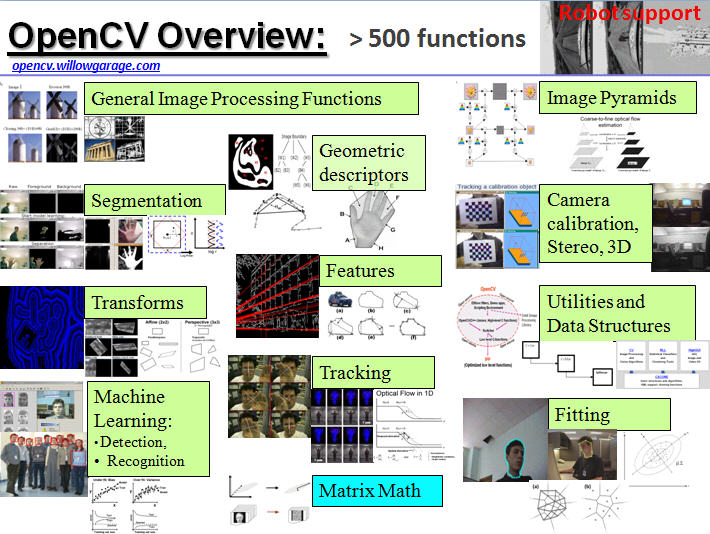
\includegraphics[width=0.75\textwidth]{Figuras/OpenCVOverview.png}
\end{figure}
\end{frame}

\begin{frame}\frametitle{Convolución}
  Si se conoce la respuesta al impulso $H(x,y)$ de un sistema SLID, se puede obtener la salida $O(x,y)$ ante cualquier entrada $I(x,y)$, mediante la convolución, definida como:
  \[O(x,y) = I(x,y)*H(x,y) = \sum_{i=-\infty}^\infty \sum_{j=-\infty}^\infty I(i,j)H(x-i, y-j)\]
  Ejemplos:
  \[\left[\begin{tabular}{cccc}
      3 & 1 & 4 & 1\\
      5 & 9 & 2 & 6\\
      5 & 3 & 5 & 8\\
      9 & 7 & 9 &3
    \end{tabular}\right]* [1\quad -1] =
  \left[\begin{tabular}{ccccc}
      3 & -2 & 3 & -3 & -1\\
      5 & 4 & -7 & 4 & -6\\
      5 & -2 & 2 & 3 & -8\\
      9 & -2 & 2 & -6 & -3
    \end{tabular}\right]\]

  \[\left[\begin{tabular}{cccc}
      3 & 1 & 4 & 1\\
      5 & 9 & 2 & 6\\
      5 & 3 & 5 & 8\\
      9 & 7 & 9 &3
    \end{tabular}\right]* \left[\begin{tabular}{c}1 \\ -1\end{tabular}\right] =
  \left[\begin{tabular}{cccc}
      3 & 1 & 4 & 1\\
      2 & 8 & -2 & 5\\
      0 & -6 & 3 & 2\\
      4 & 4 & 4 & -5\\
      -9 & -7 & -9 & -3
    \end{tabular}\right]\]
\end{frame}

\begin{frame}\frametitle{El filtro Gaussiano}
  Una primera aplicación de una convolución es el filtro Gaussiano
  \[
    g(x,y) = \frac{1}{2\pi\sigma^2}e^{-(x^2 + y^2)/(2\sigma^2)}
  \]
  Se utiliza para reducir el tipo de ruido más común que es el ruido Gaussiano. Un ejemplo de kernel Gaussiano es:
  \[ H = \frac{1}{16}
  \left[\begin{tabular}{ccc}
      1 & 2 & 1\\
      2 & 4 & 2\\
      1 & 2 & 1
  \end{tabular}\right]
\]
\end{frame}

\begin{frame}\frametitle{Gradiente}
  El gradiente de una imagen está definido como:
  \[\nabla I = \left[\frac{\partial I}{\partial x}, \frac{\partial I}{\partial y}\right]\]
  Las derivadas parciales se puede aproximar mediante diferencias finitas:
  \begin{eqnarray*}
    \frac{\partial I}{\partial x} &=& \lim_{\Delta x \rightarrow 0}\frac{I(x + \Delta x, y) - I(x,y)}{\Delta x}\approx I_{i,j} - I_{i,j-1}\\
    \frac{\partial I}{\partial y} &=& \lim_{\Delta y \rightarrow 0}\frac{I(x, y + \Delta y) - I(x,y)}{\Delta y}\approx I_{i,j} - I_{i-i,j}
  \end{eqnarray*}
  donde $(i,j)$ representan las coordenadas de imagen renglón-columna. Estas diferencias finitas se puede obtener mediante una convolución:
  \begin{eqnarray*}
    \frac{\partial I}{\partial x} &\approx& I * [1\quad -1]\\
    \frac{\partial I}{\partial y} &\approx& I * \left[\begin{tabular}{c}1\\-1\end{tabular}\right]
  \end{eqnarray*}
\end{frame}

\begin{frame}\frametitle{Gradiente}
  Una mejor aproximación de la derivada es no solo tomar la diferencia entre el valor actual y el anterior $(I_{i,j} - I_{i-1,j})$, sino promediarlo con la diferencia $(I_{i+1,j} - I_{i,j})$:
  \[\frac{1}{2}[(I_{i,j} - I_{i-1,j}) + (I_{i+1,j} - I_{i,j})] = \frac{1}{2}(I_{i+1,j} - I_{i-1,j})\]
  Generalmente se ignora el coeficiente y se utilizan los siguientes Kernels:
  \begin{eqnarray*}
    \frac{\partial I}{\partial x} &\approx& I * [1\quad 0\quad -1]\\
    \frac{\partial I}{\partial y} &\approx& I * \left[\begin{tabular}{c}1\\ 0\\-1\end{tabular}\right]
  \end{eqnarray*}
\end{frame}

\begin{frame}\frametitle{El filtro de Sobel}
  El Operador de Sobel o Filtro de Sobel consiste en un Kernel que permite obtener las derivadas parciales, aproximadas por diferencias finitas, y promediadas con un filtro Gaussiano:
  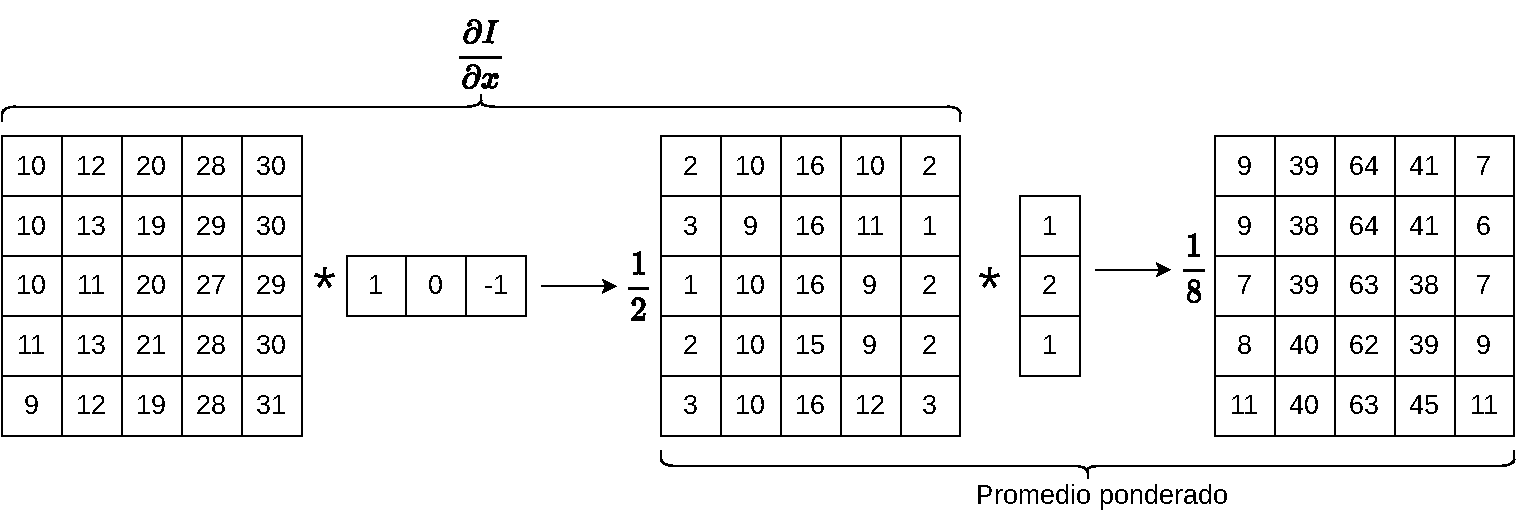
\includegraphics[width=\textwidth]{Figuras/SobelX1.pdf}
  Se realiza un proceso similar para la derivada parcial en $Y$. Aplicando la propiedad asociativa de la convolución, se obtienen los siguientes ekernels:
  \[S_x = \left[\begin{tabular}{ccc}1 & 0 & -1\\2 & 0 & -2\\1 & 0 & -1 \end{tabular}\right]\qquad\qquad
  S_y = \left[\begin{tabular}{ccc}1 & 2 & 1\\0 & 0 & 0\\-1 & -2 & -1 \end{tabular}\right]\]
\end{frame}

\begin{frame}\frametitle{Magnitud y Ángulo}
  El gradiente en cada pixel de la imagen se puede calcular mediante la approximación de las derivadas parciales:
  \begin{eqnarray*}
    \frac{\partial I}{\partial x} &\approx& I * Sx = G_x\\
    \frac{\partial I}{\partial y} &\approx& I * Sy = G_y\\
  \end{eqnarray*}
  En la mayoría de las aplicaciones es más últil expresar el gradiente en forma polar:
  \[ \nabla I = G_m \angle G_a \]
  Donde la magnitud del gradiente y la fase, para cada pixel, se calculan como:
  \begin{eqnarray*}
    G_{m_{i,j}} &=& \sqrt{G_{x_{i,j}}^2 + G_{y_{i,j}}^2}\\
    G_{a_{i,j}} &=& \atantwo(G_{y_{i,j}}, G_{y_{i,j}})\\
  \end{eqnarray*}
  Otra forma de calcular la magnitud del gradiente es mediante la norma 1:
  \[G_{m_{i,j}} = \left|G_{x_{i,j}}\right| + \left|G_{y_{i,j}}\right|\]
\end{frame}

\begin{frame}[containsverbatim]\frametitle{Ejercicio 02 - Gradiente de una imagen}
  \begin{enumerate}
  \item Abra una terminal y ejecute la simulación con el comando:
    \begin{lstlisting}[language=bash,numbers=none]
roslaunch eir2024 navigation_no_obstacles.launch
    \end{lstlisting}
  \item En otra terminal, ejecute el ejercicio dos con el siguiente comando:
    \begin{lstlisting}[language=bash,numbers=none]
rosrun eir2024 exercise02.py
    \end{lstlisting}
  \item Detenga el ejercicio 02, abra el archivo fuente y agregue el siguiente código en la línea 25:
    \begin{lstlisting}[language=Python,firstnumber=25]
grad_x = cv2.Sobel(gray, cv2.CV_16S, 1, 0, ksize=3)
grad_y = cv2.Sobel(gray, cv2.CV_16S, 0, 1, ksize=3)
abs_grad_x = cv2.convertScaleAbs(grad_x)
abs_grad_y = cv2.convertScaleAbs(grad_y)
grad = cv2.addWeighted(abs_grad_x, 0.5, abs_grad_y, 0.5, 0)
cv2.imshow("Gradient Magnitude", grad)
    \end{lstlisting}
  \item Corra nuevamente el ejercicio y observe el resultado. Ahora agregue el siguiente código en la línea 21:
    \begin{lstlisting}[language=Python,firstnumber=21]
gray = cv2.GaussianBlur(gray, (5, 5), 0)
    \end{lstlisting}
  \item Corra nuevamente el ejercicio 2 y observe el resultado. 
  \end{enumerate}
\end{frame}

\begin{frame}\frametitle{Detector de Bordes de Canny}
  El detector de bordes de Canny es un detector basado en gradiente que consta de los siguientes pasos básicos:
  \begin{enumerate}
  \item Obtención del gradiente en magnitud y ángulo, mediante operadores de Sobel
  \item Supresión de puntos no máximos
  \item Aplicación de un doble umbral
  \end{enumerate}
  Aunque no es un paso en sí del Detector de Canny, generalmente se considera como primer paso la aplicación de un filtro Gaussiano para disminuir el ruido. 
\end{frame}

\begin{frame}\frametitle{Obtención del gradiente}
  Después del filtro Gaussiano, el primer paso es obtener el gradiente de la imagen mediante el Filtro de Sobel, en la forma de magnitud y ángulo:\\
  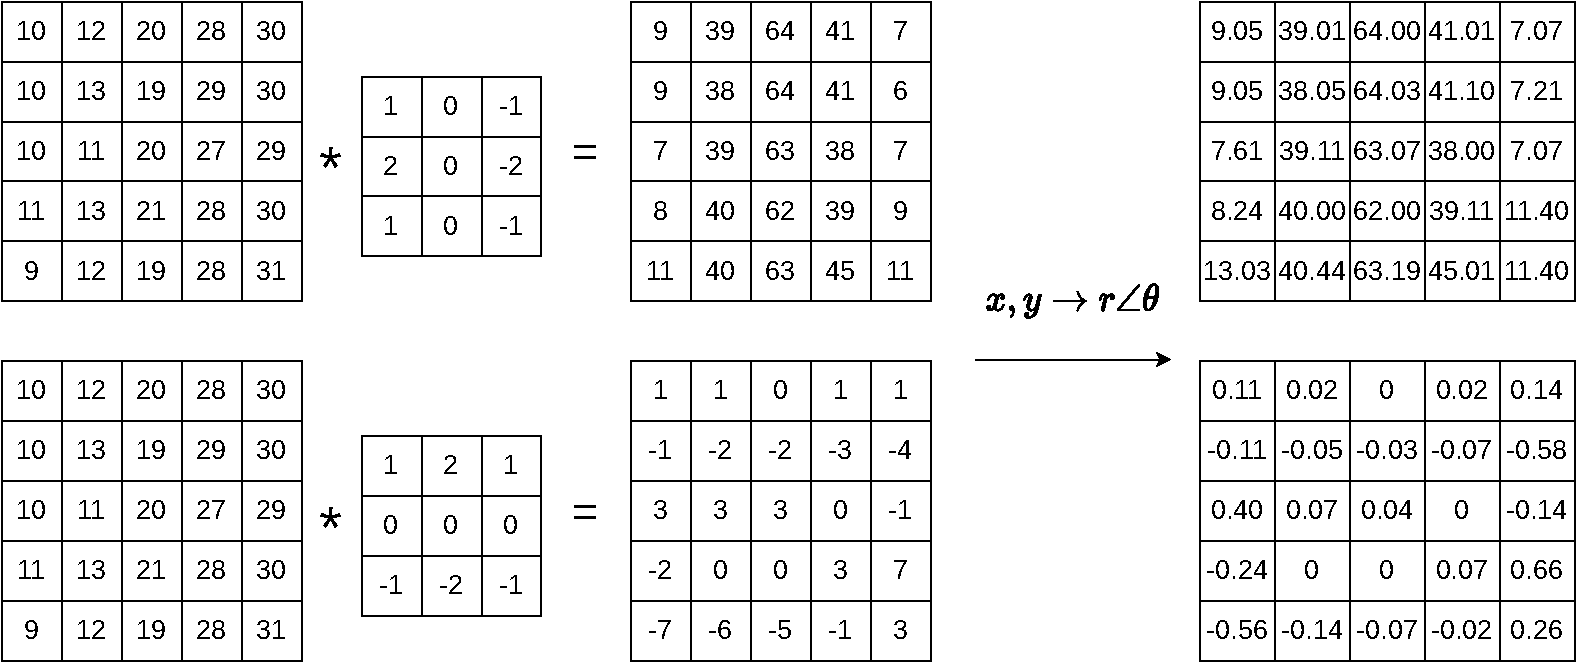
\includegraphics[width=0.9\textwidth]{Figuras/SobelXY.pdf}
\end{frame}

\begin{frame}\frametitle{Supresión de no máximos}
  Este paso consiste en comparar la magnitud de cada pixel, con los pixeles anterior y posterior en la dirección del gradiente.
  Aunque la fase es un ángulo en $[-\pi, \pi]$, la dirección del gradiente se debe redondear a algún valor correspondiente a la connectividad 8: \textit{N, NE, E, SE}. Debido a que el pixel se compara en la dirección positiva y negativa del gradiente, no es necesario considerar las direcciones \textit{S, SW, W, NW}.
  \begin{figure}
    \centering
    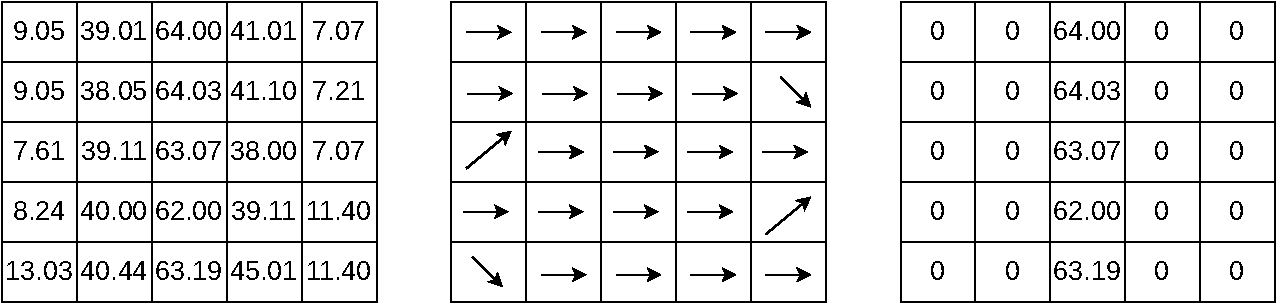
\includegraphics[width=0.9\textwidth]{Figuras/SobelMA.pdf}
  \end{figure}
  Para cada pixel $p_i$, considere $p_{i+1}$, el pixel siguiente en la dirección del gradiente, y $p_{i-1}$, el pixel anterior, en la dirección del gradiente. El valor para cada pixel $q_i$ en la imagen resultante es:
  
  \[q_i = \begin{cases}p_i\qquad\qquad\textrm{si}\qquad p_i > p_{i+1} \qquad\textrm{y}\qquad p_i > p_{i-1}\\
  0\qquad\qquad\textrm{en otro caso}\end{cases}\]
\end{frame}

\begin{frame}\frametitle{Aplicación de doble umbral}
  En este paso, se definen dos umbrales: superior $\theta_u$ e inferior $\theta_l$. Los pixeles se clasifican en tres tipos:
  \begin{itemize}
  \item Fuertes: pixeles con magnitud del gradiente mayor que el umbral superior $|\nabla | > \theta_u$
  \item Débiles: pixeles con magnitud del gradiente entre ambos umbrales $\theta_l < |\nabla| < \theta_u$
  \item Suprimidos: pixeles con magnitud del gradiente menor que el umbral inferior $|\nabla| < \theta_l$
  \end{itemize}
  La imagen resultante se forma con las siguientes reglas:
  \begin{itemize}
  \item Todos los pixeles fuertes son parte de un borde.
  \item Todos los pixeles suprimidos no son bordes. 
  \item Los pixeles débiles son parte de un borde solo si están conectados (en conectividad 8) con un pixel fuerte.
  \end{itemize}
  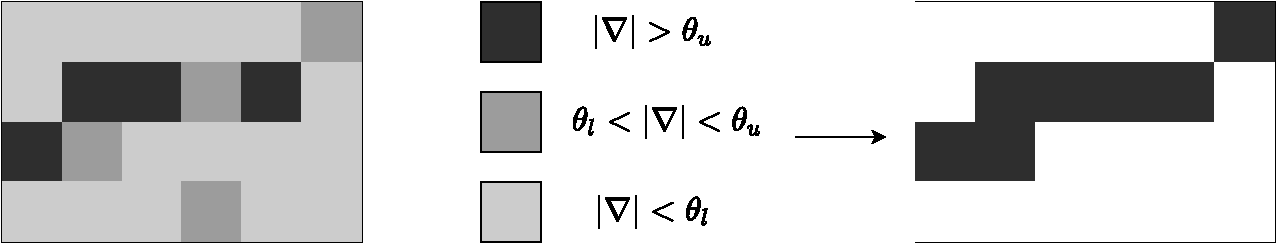
\includegraphics[width=\textwidth]{Figuras/DoubleThreshold.pdf}
\end{frame}

\begin{frame}[containsverbatim]\frametitle{Ejercicio 03 - Detección de Bordes}
  \begin{enumerate}
  \item Abra una terminal y ejecute la simulación con el comando:
    \begin{lstlisting}[language=bash,numbers=none]
roslaunch eir2024 navigation_no_obstacles.launch
    \end{lstlisting}
  \item Abra el archivo fuente del ejercicio 03 y agregue el siguiente código en la línea 33:
    \begin{lstlisting}[language=Python, firstnumber=33]
gray = cv2.GaussianBlur(gray, (5,5), 0)
edges = cv2.Canny(gray, lower_threshold, upper_threshold)
    \end{lstlisting}
  \item En otra terminal, ejecute el ejercicio 03 con el siguiente comando:
    \begin{lstlisting}[language=bash,numbers=none]
rosrun eir2024 exercise03.py
    \end{lstlisting}
  \item Sintonice los umbrales hasta obtener una detección de bordes satisfactoria. Utilice la GUI para mover el vehículos y probar en diferentes condiciones. 
  \end{enumerate}
\end{frame}

\begin{frame}\frametitle{La Transformada Hough}
  La Transformada Hough es un método que permite encontrar líneas, círculos y otras formas geométricas que se puedan describir fácilmente mediante expresiones analíticas. En el caso de las líneas, se trata de encontrar los dos parámetros que describen la recta:
  \begin{columns}
    \begin{column}{0.4\textwidth}
      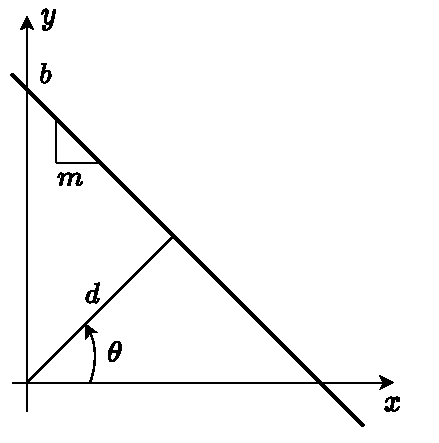
\includegraphics[width=\textwidth]{Figuras/Hough2.pdf}
    \end{column}
    \begin{column}{0.6\textwidth}
      \begin{itemize}
      \item La forma pendiente-ordenada $y = mx + b$ tiene la desventaja de no poder expresar líneas verticales.
      \item La forma canónica $Ax + By + C$ requiere de una normalización $A_1 x + B_1 y + 1 = 0$ para que solo sean dos parámetros.
      \item Una forma más conveniente, es la forma normal $d = x\cos\theta + y\sin\theta$
      \item Esta última forma tiene una ventaja: si la línea correponde a un borde, el ángulo $\theta$ será la dirección del gradiente. 
      \end{itemize}
    \end{column}
  \end{columns}
\end{frame}

\begin{frame}\frametitle{El Espacio de Hough}
  El Espacio de Hough, para el caso de las líneas, es el conjunto de todos los posibles pares $(\theta, d)$.
  \begin{itemize}
  \item Una recta $L$ en el espacio cartesiano corresponde a un punto $P_h$ en el Espacio de Hough
  \item Un punto $P_c$ en el espacio cartesiano corresponde a una curva $C$ en el Espacio de Hough. Esta curva representa los parámetros $(\theta_i, d_i)$ de todas las rectas $L_i$ que pasan por el punto $P$.
  \end{itemize}
  \begin{figure}
    \centering
    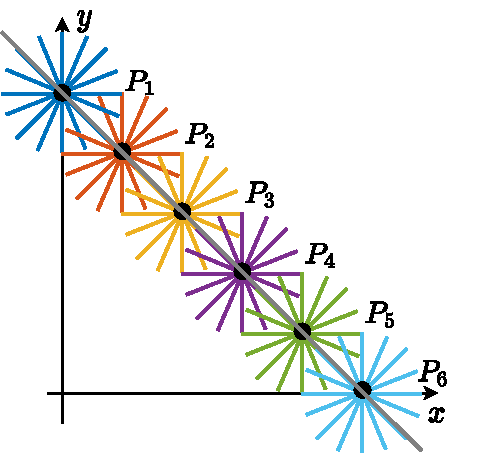
\includegraphics[width=0.35\textwidth]{Figuras/Hough1.pdf}
    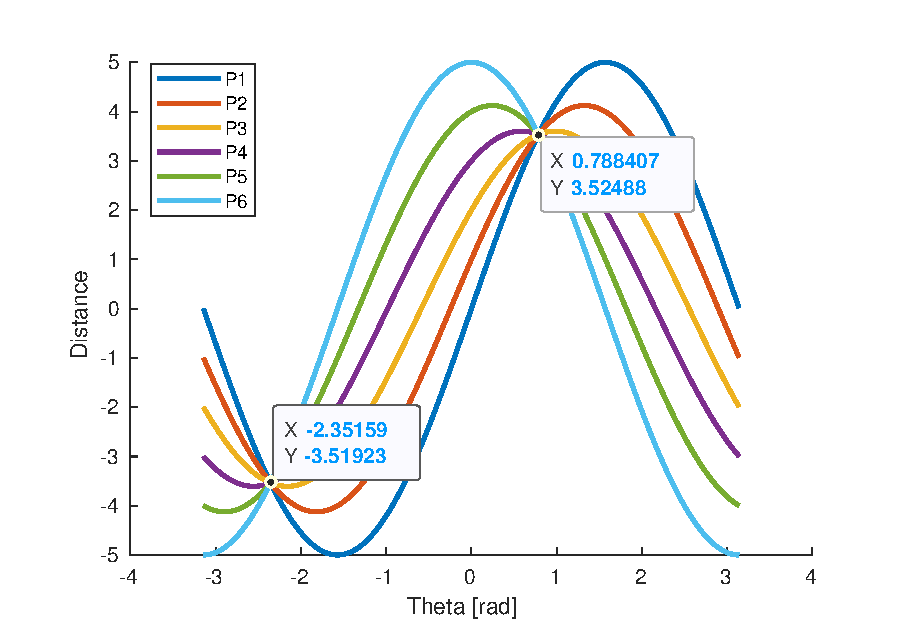
\includegraphics[width=0.5\textwidth]{Figuras/Hough1.eps}
  \end{figure}
\end{frame}

\begin{frame}\frametitle{Extracción de Líneas por Transformada Hough}
  Este método consiste en encontrar las curvas $C_i$ en el espacio de Hough que pasan por cada punto $P_c$ en el espacio cartesiano. Los puntos $P_h$ en el Espacio de Hough por donde pasen más curvas $C_i$ corresponderán a las rectas resultantes en el espacio cartesiano.
  \begin{figure}
    \centering
    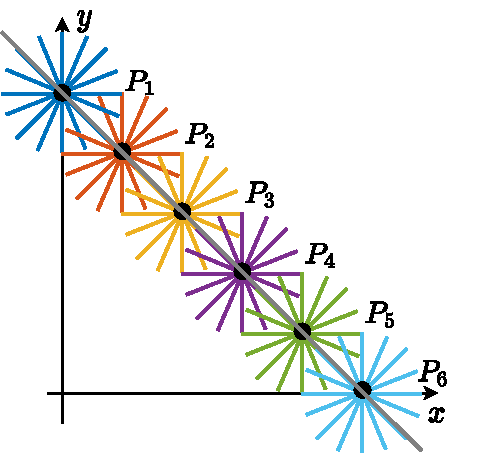
\includegraphics[width=0.35\textwidth]{Figuras/Hough1.pdf}
    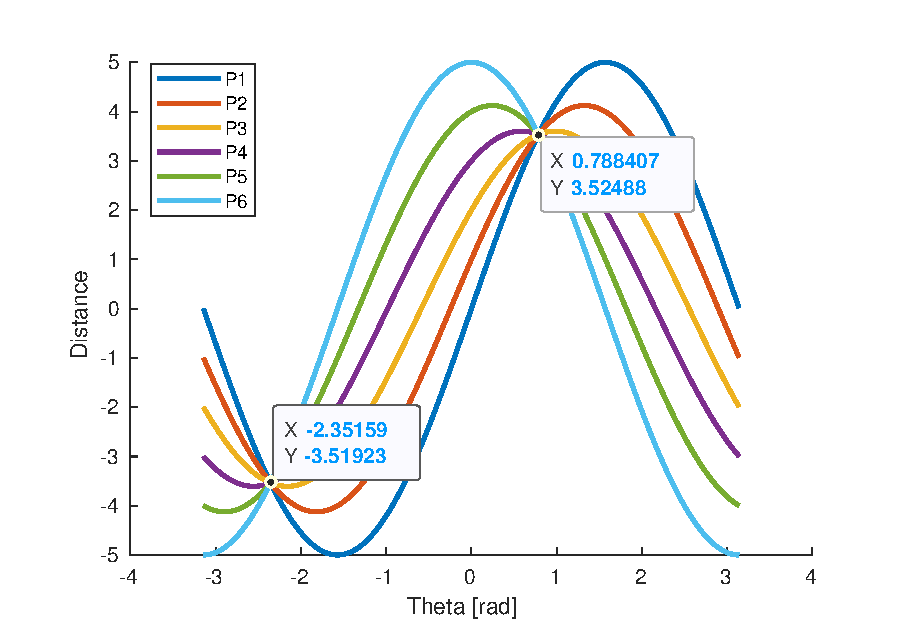
\includegraphics[width=0.5\textwidth]{Figuras/Hough1.eps}
  \end{figure}
\end{frame}

\begin{frame}\frametitle{Extracción de Líneas por Transformada Hough}
  \begin{algorithm}[H]
    \KwIn{Imagen binaria $M$, umbral mínimo de votos $a_{min}$}
    \KwOut{Líneas expresadas en la forma $(d,\theta)$}
    \DontPrintSemicolon
    \;
    Inicializar en 0 un conjunto $A$ de acumuladores para cada par cuantizado $(d_k,\theta_k)$\;
    \ForAll{Pixel $M[i,j] \neq 0$}
    {
      \ForAll{Ángulo $\theta_k$ cuantizdo}
      {
        $d = j\cos\theta_k + i\sin\theta_k$
        $d_k = $ valor cuantizado de $d$
        Incrementar en uno el acumulador correspondiente $A[d_k, \theta_k]$
      }
    }
    \ForAll{$a \in A$}
    {
      \If{$a > a_{min}$}
      {
        Agregar la línea $(d_k, \theta_k)$ al conjunto de líneas detectadas
      }
    }
    Devolver el conjunto de líneas detectadas
  \end{algorithm}
\end{frame}

\begin{frame}[containsverbatim]\frametitle{Ejercicio 04 - Detección de líneas}
  \begin{enumerate}
  \item Abra una terminal y ejecute la simulación con el comando:
    \begin{lstlisting}[language=bash,numbers=none]
roslaunch eir2024 navigation_no_obstacles.launch
    \end{lstlisting}
  \item Abra el archivo fuente del ejercicio 04 y agregue el siguiente código en la línea 45:
    \begin{lstlisting}[language=Python, firstnumber=45]
gray = cv2.GaussianBlur(gray, (5,5), 0)
edges = cv2.Canny(gray, 50, 150)
lines = cv2.HoughLinesP(edges, 2, numpy.pi/180, hough_threshold, minLineLength=min_length, maxLineGap=max_gap)
draw_lines(lines, img)
    \end{lstlisting}
  \item En otra terminal, ejecute el ejercicio 04 con el siguiente comando:
    \begin{lstlisting}[language=bash,numbers=none]
rosrun eir2024 exercise04.py
    \end{lstlisting}
  \item Sintonice las constantes hasta obtener una detección de líneas satisfactoria. Utilice la GUI para mover el vehículos y probar en diferentes condiciones. 
  \end{enumerate}
\end{frame}

\begin{frame}\frametitle{Detección de carriles}
  En el ambiente se pueden detectar varias líneas pero no todas son bordes de carriles:
  \begin{figure}
    \centering
    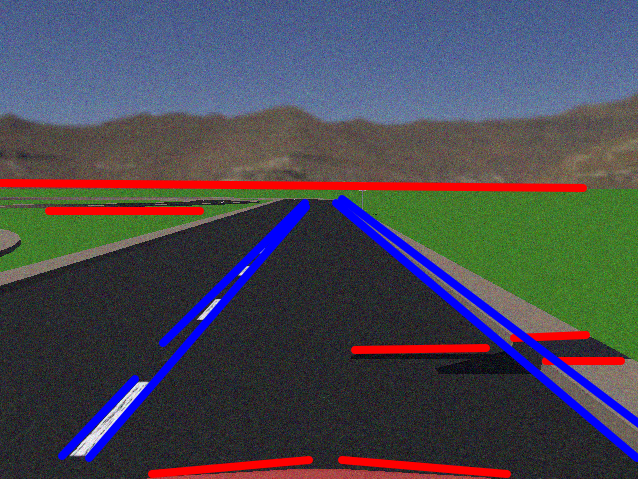
\includegraphics[width=0.5\textwidth]{Figuras/LineFiltering.png}
  \end{figure}
  \begin{itemize}
  \item Los bordes de los carriles no pueden ser horizontales cerca del auto
  \item En un terreno plano no pueden estar por arriba del horizonte
  \item Se puede hacer un promedio ponderado de las líneas detectadas
  \item Es mejor tomar como origen el centro del frente del vehículo 
  \end{itemize}
\end{frame}

\begin{frame}[containsverbatim]\frametitle{Ejercicio 05 - Detección de carriles}
  
\end{frame}
\section{Seguimiento de carriles}

\begin{frame}\frametitle{Modelo cinemático}
  Considere la base móvil de la figura:
  \begin{figure}
    \centering
    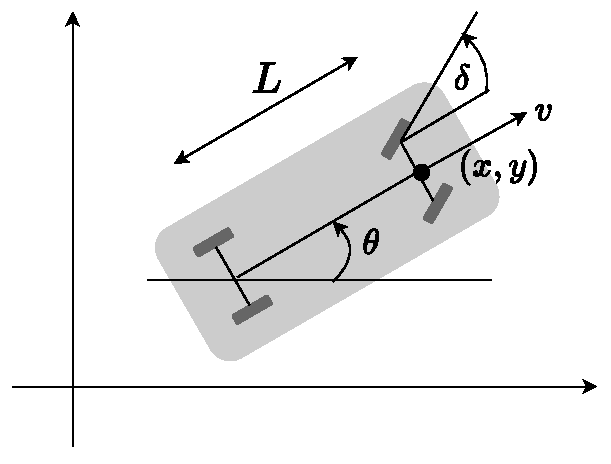
\includegraphics[width=0.3\textwidth]{Figuras/Ackermann.pdf}
  \end{figure}
  con
  \begin{itemize}
  \item $(x,y,\theta)$ la configuración en el plano de movimiento, considerando como centro el centro del eje delantero (tracción delantera)
  \item $L$ la distancia entre ejes de las llantas
  \item $v$ es la velocidad lineal del vehículo considerada como señal de entrada
  \item $\delta$ es el ángulo de las llantas delanteras (volante) también considerada como señal de control
  \end{itemize}
  El objetivo es determinar $v$ y $\delta$ de modo que le vehículo tenga determinado comportamiento.
\end{frame}

\begin{frame}\frametitle{Seguimiento de carriles}
  El seguimiento de carriles se puede hacer con base en las líneas detectadas. Considere la figura:
  
\end{frame}
% \input{Tex/Vision.tex}
% \input{Tex/Manipulacion.tex}
% \input{Tex/SintesisVoz.tex}
% \input{Tex/ReconocimientoVoz.tex}
% \input{Tex/Planeacion.tex}
\bibliographystyle{abbrv}
\bibliography{References}
\begin{frame}
  \Huge{Gracias}
  \[\]
  \Large{Contacto}
  \[\]
  \large
  Dr. Marco Negrete\\
  Profesor Asociado C\\
  Departamento de Procesamiento de Señales\\
  Facultad de Ingeniería, UNAM.
\[\]
mnegretev.info\\
marco.negrete@ingenieria.unam.edu\\
\end{frame}
\end{document}
